\chapter{Implementation}
\label{chap:implementation}

This chapter is devoted to the implementation of our software.
The result of this work is an Android application that allows to take photos with a camera, browse them and pick a pair of images for the resulting 3D model of the disparity map which was calculated from the selected input data.
The expected input data are described in Section \ref{prob}.

Our task was to design an algorithm solving the problem of calculation the depth information from a pair of images on the Android platform.
When implementing the software for Android we are limited to the input data of lower quality.
The Android camera lenses are made of plastic and cause a significant non-linear distortion which can not be easily simulated.
Also, due to the limited capacity of calculation memory of mobile phones we need to down-sample the resolution of the input images.
These problems disallow using common approaches of solving the dens corresponding problem.

In Section \ref{sec:impl_outline} of this chapter we enumerate the subtasks and describe how was our approach designed.
 
\section{Implementation outline}
\label{sec:impl_outline}
In the this section we describe the way how was the task solved, what algorithms were chosen and how was the application implemented.
%To implement the Android application, several subtask must be completed.
%At first it is the graphical user interface and handling the camera which is managed through Android Activities and xml files as we described in chapter \ref{chap:android}.
%Secondly, we deal with the calculation, which consist of the image registration, the keypoint detection, the keypoint matching and solving the dense correspondence problem.

To solve our task, we followed these steps:
\begin{itemize}
\item at first we find the initial relative position of the pair of input images,
\item then we detect and match SURF keypoints from which is chosen the most robust match to specify more accurate relative position,
\item then we detect larger amount of SURF keypoints. The matching process uses the information of the relative position estimated in the previous step,
\item at last, we get the dense correspondences by detecting even more matches using the optical flow algorithm.
\end{itemize}

Finding the initial relative position of the pair of the images is implemented by using Sum of absolute differences (described in Section \ref{sec:metrics}).
At first, we create a scale-space, find the overlap of the images in the lowest scale and by upscaling specify the overlapping area more accurately.
In this way the registration runs in approximately two seconds for a pair of the expected input.

%Image registration (finding the relative position of the pair of the images) is implemented by using Sum of absolute differences (described in \ref{sec:metrics}).
%At first, we create a scale-space from the input pair of images, so we can find relatively fast the overlap with minimal difference of intensities of the image pair by comparing each possible overlap in the lowest scale. 
%When we have the approximate overlap, we take the image of the scale above and try to find better result by shifting the matched area in the 5-pixels range.
%This we repeat until we look over all of the levels of the scale-space or for computational efficiency we estimate the result satisfiable when the width or hight of the investigating scale image is higher then a constant value.
%Because we expect the image input in the size of approximately 1000 $\times$ 800 pixels, for the experiments in our work we set the constant to 200. 

\begin{figure}[h]
\centerline{
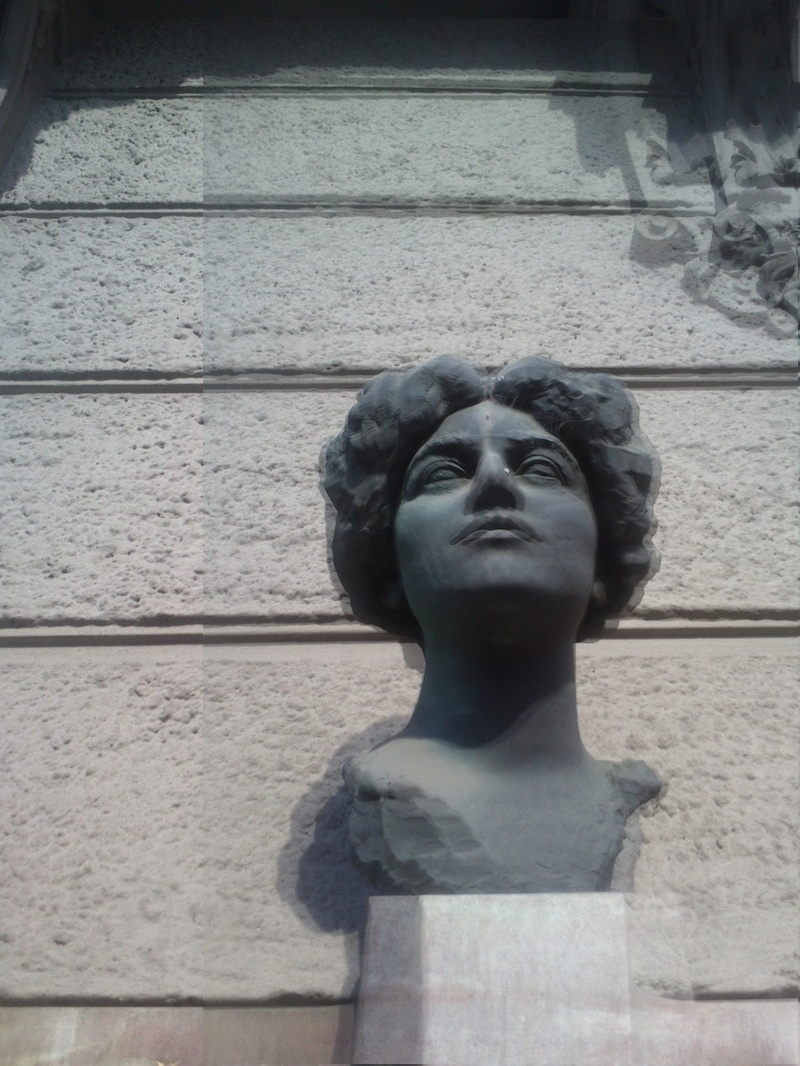
\includegraphics[width=4.5cm]{img/ema_overlap.png}
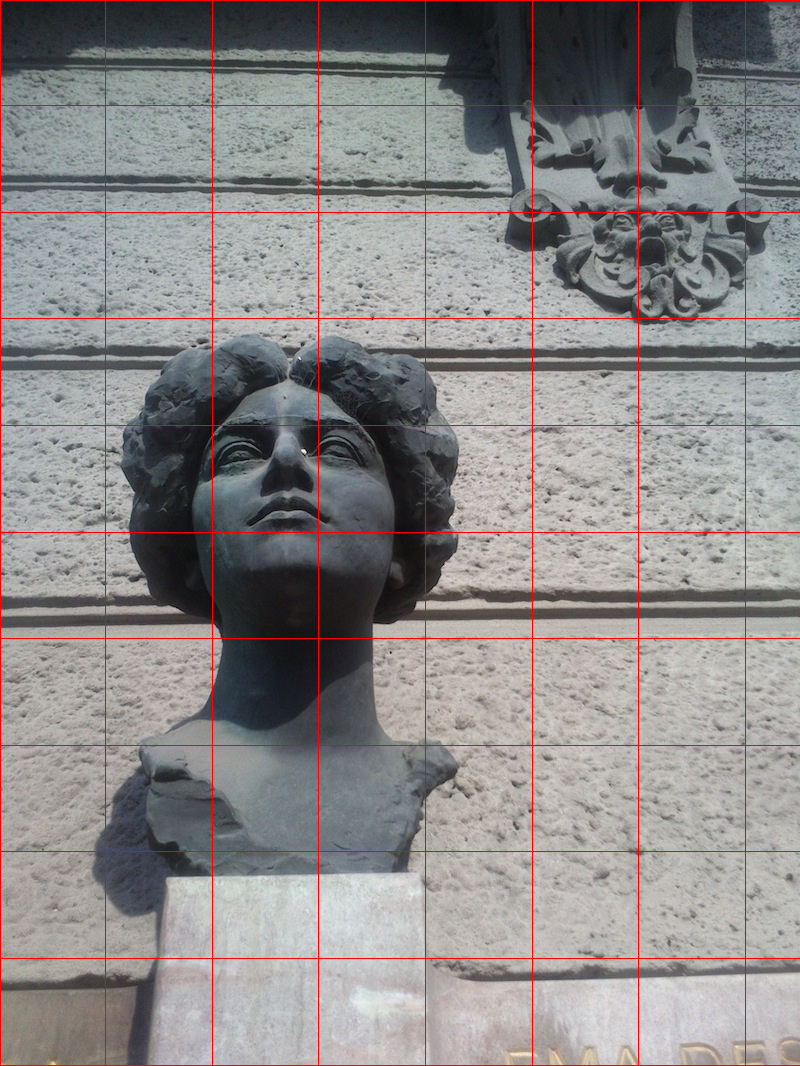
\includegraphics[width=4.5cm]{img/ema_buckets.png}}
\caption{Left: The result of the registration where the process of upscaling was stopped when the height of the image was over 200px. Right: The division of an image into square-boxes.}
\label{fig:overlap_and_buckets}
\end{figure}

The next step of the process is detection of keypoints which are detected with the SURF detector.
We divide the images into square-boxes of the same size and to each square-box we assign an array of keypoints situated in it.
This saves the computational time when finding the match -- instead of comparing every possible correspondence between the images we compare only those which are situated in the square-boxes located in the corresponding areas.
At first we find the most robust match from only the SURF keypoints where the response is higher than 4000.
Based on this match we estimate the direction of the shift which gives us more accurate relative position of the input pair of images.

%The next step of the process is detection of keypoints which are detected with the SURF detector.
%We divide the images into square-boxes of the same size and to each square-box we assign an array of keypoints situated in it.
%Because of the previous calculation of approximate overlap we do not have to match all keypoints in the image, but we choose only the keypoints lying in the overlap.
%To identify the relative position of the image pair better we detect the most robust keypoint match from our SURF keypoint set and calculate the vector defining the direction of the shift of the keypoint.
%To find this robust match we choose only the keypoints with response higher than 4000 and each of them we try to match with one keypoint extracted in the second image but only in the corresponding 30 $\times$ 30 pixels area determined due the previous image registration.
%To decrease the computational time we use the pre-calculated square-boxes to find the keypoints of the second image lying in this area.
%To avoid mismatches we reject the matches where the matched keypoints differs too much in the orientation or if there is more than one obvious potential points for the match.

\begin{figure}[h]
\centerline{
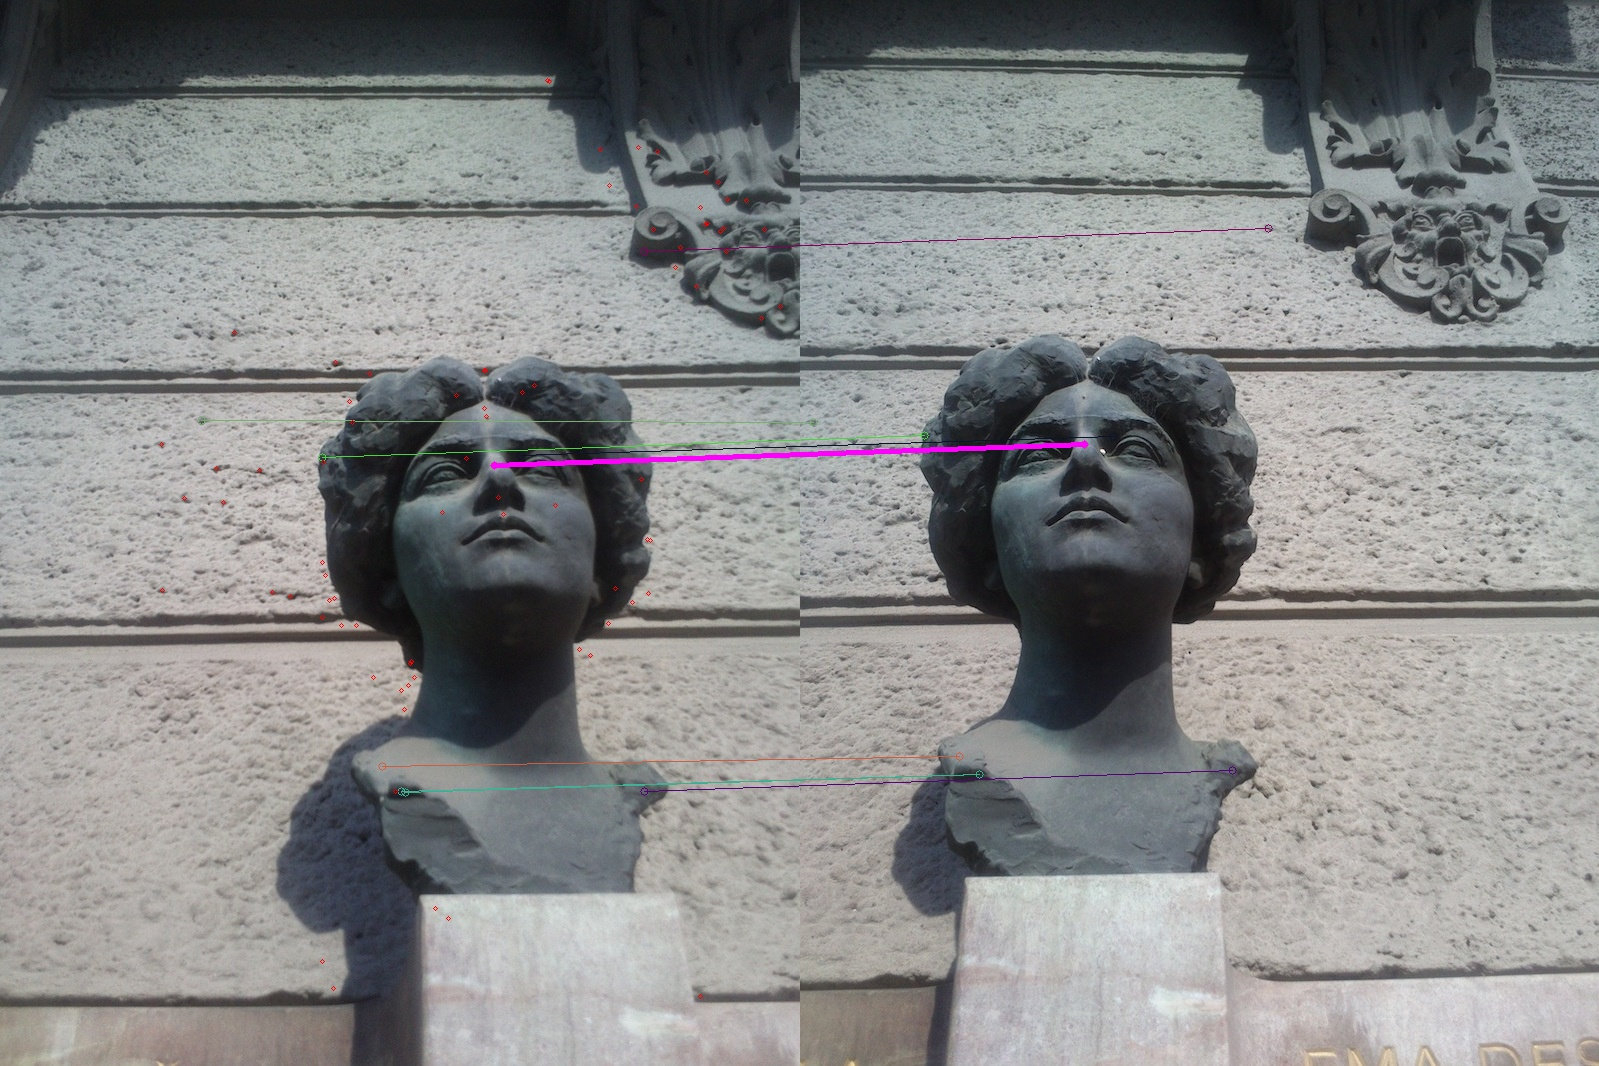
\includegraphics[width=9cm]{img/ema_direction.png}}
\caption{The most robust match chosen from the keypoints with response higher than 4000. According to this match the more accurate relative position of images is estimated.}
\label{fig:robust_match}
\end{figure}

In the next step we match the detected SURF keypoints one more time.
For each keypoint we calculate the corresponding area of the surroundings in the shape of a rectangle oriented in the direction of the shift. 
To avoid mismatches we reject the matches where the matched keypoints differs too much in the orientation or if there is more than one obvious potential points for the match.

%When we know the more accurate relative position of the images, we investigate the keypoints one more time.
%Now we iterate all of them. 
%Each keypoint in the first image we try to match with a keypoint in the estimated corresponding surrounding area in the second image in the shape of oriented rectangle computed based on the more accurate relative image position.
%This oriented rectangle actually consists of two rectangles -- one large and one smaller localised in the middle of the previous one.
%The corresponding keypoint is accepted only if its located in the inner one.
%The size of the larger rectangle is set to 60 $\times$ 120 pixels.
%The inner rectangle after some experiments was set to the 10\% of width and 20\% of height.
%It was shown that it gives better results than only a bit larger window of the the width of 20\% of width and 35\% of height size.
%Matched keypoints which differs too much in the orientation or are not obviously the best match we reject again.
%We can see the comparison in Figure \ref{fig:matching_comparison}.


%Dense correspondence: optical flow::
At this point we have relatively robust matches for sparse correspondence. 
For the calculation of the depth information we need to extract more corresponding points.
Assuming the difference of images is limited, we use for this purpose optical flow algorithm. 
For each SURF keypoint in the first image we detect corners or other features acceptable for the tracking algorithm in its 70 $\times$ 70 pixels area.


Calculating the optical flow we get the corresponding points in the second image.
With high probability some of the results will be influenced by noise.
To avoid these mismatches we calculate the variation of the distances between each match.
If the variation is higher than 300 we discard all of the detected optical flow matches.

The result is visualized in OpenGL ES.
Every keypoint is represented as a triangle in a space with the depth calculated from the correspondence.
At first, the user can view the rough model created from the results of SURF matching.
Each time some of the dense corresponding points are calculated with optical flow algorithm, the model is updated.


